\chapter{Firmware Design}

Software has a critical impact on hardware design. Typically, for a project like this, either ContikiOS or TinyOSwould be chosen. Both of them are componentized operating systems that are the de-facto standard in wireless embedded systems research. However, neither was used for this project. Instead, the board runs a port of the QP Framework\cite{Samek2008}, an event-based actor framework combined with a very simple, cooperative multitasking kernel. The advantage of choosing the QP Framework is that the cooperative kernel can be swapped out for a pre-emptive kernel in the future depending on application requirements for hard real-time guarantees. No such capability is supported by TinyOS or ContikiOS, because of the resource constraints imposed by the platforms they must support.

As a result of running directly on the microcontroller, there is very little hardware abstraction; peripherals and MCU features must be directly programmed and accessed via the ROM functions provided by the manufacturer. New events are easily created and assigned to the QP scheduler, which schedules all tasks in a run-to-completion fashion. Given that no functionality required real-time scheduling, a cooperative run-to-completion kernel was selected. It is simple to implement, uses less stack and memory space, and does not suffer from the complexity of traditional preemptive real-time operating systems.

\section{Standard Firmware Operation}

The standard firmware load for the board consists of an always on HTTP server that reports sensor data according to HTTP get requests. The use-case for most of the ecoMOD boards has been to support mains-powered operation. Batteries, no matter how good, eventually self-discharge. Obtaining permission to replace sensor batteries while the house is being occupied has historically been difficult on occasion.  In addition, mains-powered operation allows for over-the-air updates to be applied to the firmware if necessary in an easy fashion.

\begin{figure}[h]
\centering
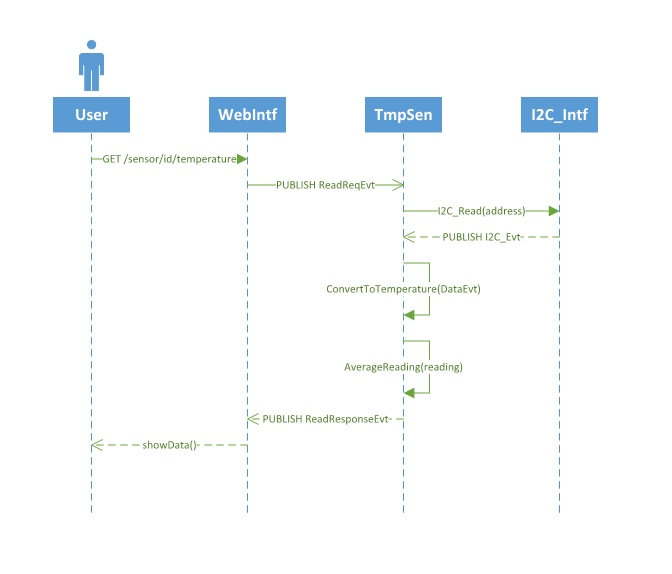
\includegraphics[width=0.7\linewidth]{images/softwareflow}
\caption[Firmware Event Timeline]{Typical Event Timeline for Default Firmware}
\label{fig:softwareflow}
\end{figure}

\section{Battery-Powered Operation}

A low-power firmware load was developed for experimental purposes. The node firmware design for the battery powered case is based on the following low duty cycle principle: the node is asleep for the majority of the time, wakes up quickly on an sensor data acquisition event, processes the data, stores the data in a buffer , and then returns to sleep. If the buffer is full, it takes the data and posts it to an arbitrary URL. 

Wireless transmission and receive are the dominant power consumers in most battery-powered devices. The board designed here is no exception, with energy consumption dominated by the transceiver. In fact, the MCU consumes 3 to 6 mA of current while active, compared to 275 mA by the radio in full power transmit mode. It is clear that the energy consumption bottleneck lies in the wireless radio. Several techniques can be used here to reduce power consumption: compressing the data stream, and employing burst transmissions.

\subsection{Burst Transmission}

A wireless sensor node spends most of time engaged in one-way communication. Very rarely does it need to be actively listening for commands from another device. If the node collects data at a fixed rate, then the radio on time can be minimized by buffering as much data as possible, and then transmitting it. At all other times, the radio can be placed in a power-saving idle or sleep mode. This trades power consumption for data latency and device memory.

Let the average power drawn by the radio during bursts be defined as $P_{B}$. Then, 

\begin{equation}
P_{B} = \frac{1}{T_{B}}[E_{oh} + T_{TX} +(T_{B}-T_{TX})P_{idle}]\cite{Calhoun2005}
\end{equation}

where $T_{B}$ is the period between bursts, $E_{oh}$ is the radio on/off power toggling cost, $T_{TX}$ is the transmission time, $P_{TX}$ is the power consumed during transmission, and $P_{idle}$ is the power consumed while the radio is asleep.

From the equation, it can be seen that in the limit as $T_B$ approaches infinity, the power consumption approaches $P_idle$. Of course, an infinitely long burst period also leads to infinitely long latency and infinitely large storage. A compromise time between bursts period of 24 hours was chosen. The current board firmware load has approx. 80 kB of RAM available that can be set to persist during low-power deep sleep mode which is more than adequate (by a factor of 40) to support the storage of 16-bit samples acquired at one sample/minute. As a result, the board spends more than 98\% of its operating time in low-power deep sleep. 
